%% PACKAGES

\documentclass[journal]{IEEEtran}
\usepackage{blindtext}
\usepackage{graphicx}
\usepackage{cite}
\usepackage[cmex10]{amsmath}
\usepackage{url}

% *** SPECIALIZED LIST PACKAGES ***
%\usepackage{algorithmic}
% http://www.ctan.org/tex-archive/macros/latex/contrib/algorithms/
% http://algorithms.berlios.de/index.html
% *** ALIGNMENT PACKAGES ***
%\usepackage{array}

% correct bad hyphenation here
\hyphenation{net-works semi-conduc-tor}

\begin{document}
\title{Academic Planner}

\author{
    Delgado Ruiz, David Mauricio \texttt{dm.delgado10@uniandes.edu.co}\\ \and 
	Hernandez Cantero, Laura Sof\'ia\ \texttt{ls.hernandez10@uniandes.edu.co}\\ \and
	Mendoza Arrieta, Camilo Andres \texttt{ca.mendoza968@uniandes.edu.co}\\ \and
	Murillo Castillo, Juan Guillermo\ \texttt{jg.murillo10@uniandes.edu.co}\\ \and
  	Remolina-Guti\'errez, Maria Camila \texttt{mc.remolina197@uniandes.edu.co} 
}

\maketitle

\begin{abstract}
%\boldmath
This article presents an optimization application that helps undergraduate students of Universidad de los Andes (Colombia) that are enrolled in a double major or minor, to minimize the number of semesters required for their graduation. The application offers a detailed plan, semester by semester, with all the courses suggested to sign up for. It is also an iterative tool that takes into account the classes that the student has already approved. This article consists in the final project for the class \textit{Modelling, Simulation \& Optimization} (2017-10).
\end{abstract}

\begin{IEEEkeywords}
	optimization, semestral planning, graphs
\end{IEEEkeywords}

\section{Introduction}
The problem of academic planning by semester or quarters is something each undergraduate student has to approach when enrolled in college. However, in the majority of the cases, each major offers a suggested flow of courses per period so that the degree can be obtained in the time the university claims. \\

Nonetheless, most universities offer the possibility to perform a double major or minor during the undergraduate studies. Then, the task of planning each academic period becomes non trivial and deploys a big number of combinations between majors and minors. For this reason, and taking into account that most of the students and parents want to minimize the time and money spent for college tuition, we want to present an optimization tool that solves this problem specially for major/minor merges. \\

All of us, the authors, are undergraduate students at Universidad de los Andes (Uniandes) in Bogot\'a, Colombia. In this university, by 2015 the 30.2\% of the students were enrolled in a double major and 21\% in a minor \cite{boletinuniandes}. This means that a great portion of our school has to deal with the problem stated above. For this reason we chose our university to base the prototype of our application and to test the results of our solution. \\

\section{Problem solution}

In order to approach this problem, we started with a mathematical formulation followed by an implementation in the software GAMS. Then we created an interactive frontend website that allows to set the restrictions. Finally we run GAMS and other technologies in the backend to join all the application together. The details for each part are displayed in the next subsections. \\

\subsection{Mathematical formulation}

\subsubsection{Parameters}
In the following table we describe the conventions we will use during the article. \\

\begin{table}[h!]
	\centering
	\caption{Table of conventions}
	\label{conventions}
	\begin{tabular}{|c||l|}
		\hline
		\textbf{Symbol} & \multicolumn{1}{c|}{\textbf{Meaning}} \\ \hline
		$S$ 			& Number of semesters                   \\ \hline
		$C$				& Number of courses                     \\ \hline
        $M_{ik}$        & Adjacency matrix between courses      \\ \hline
	\end{tabular}
\end{table}

The matrix M contains the information of the merge of the all majors and minors that the student has. It is defined as:

\[ M_{ik} = 
    \begin{cases} 
      0 & \textrm{if course $i$ has no relation with course $k$} \\          
      1 & \textrm{if course $i$ is prerequisite of course $k$} \\   
      2 & \textrm{if course $i$ is corequisite of course $k$} \\  
    \end{cases}
\]\\

Where $i,k \in [1,C]$.\\

\subsubsection{Decision Variable}
The decision variable we will use is:

\[ x_{ij} = 
    \begin{cases} 
      1 & \textrm{if I take course $i$ in semester $j$} \\   
      0 & \textrm{the rest of the cases} \\  
    \end{cases}
\]

Where $i \in [1,C]$ and $j \in [1,S]$. \\

\subsubsection{Objective function}
The variable that we want to minimize is the number of semesters $n$:

\begin{equation}
\label{objectiveFunction}
n = \displaystyle\sum_{i}\sum_{j} j^5 x_{ij}
\end{equation}

\subsubsection{Constraints}
The mathematical formulation takes into account 4 basic constrains to simplify the problem:\\

\begin{itemize}
    \item A course is approved only once.
    
    \begin{equation}
        \label{noRepeats}
        \forall i, \quad \displaystyle\sum_{j=1}^{S} x_{ij} = 1
    \end{equation}
    
    \item The student sets a maximum of credits ($c_{max}$) by semester, that cannot be exceeded.
    
    \begin{equation}
        \label{maxCredits}
        \forall j, \quad \displaystyle\sum_{i=1}^{C} x_{ij} * \mathrm{credits}(i) \leq c_{max}
    \end{equation}
    
    \item If course A is a prerequisite of another course B, A has to be in a semester previous to B's.
    
    \begin{equation}
        \label{prereq}
        \textrm{if} \quad x_{ij} =1 \quad \Rightarrow \quad \forall a | M_{ai} = 1; \sum_{k=1}^{j-1} x_{ak} = 1
    \end{equation}
    
    \item If course A is a corequisite of another course B, A has to be in a semester previous or equal to B's.
    
    \begin{equation}
        \label{correq}
        \textrm{if} \quad x_{ij} =1 \quad \Rightarrow \quad \forall a | M_{ai} = 2; x_{aj} = 1
    \end{equation}
    
\end{itemize}

\subsection{Computational implementation}

For the computational implementation of the optimization, we used the software \textbf{GAMS} \cite{gams}. We treated the solution as a mixed integer linear programming problem (MIP). We selected the solver CBC. The results were finally exported as a text file. The code that shows the implementation of the optimizer with a basic example is available publicly in our GitHub repository at the URL  \url{https://github.com/projectsuniandes/planeadorsemestral_optimizador/blob/gams/optimizador.gms}.\\

After the optimizer implementation, we created a website in which the user could insert the basic restrictions and major/minor combinations of his/her choice. For this, we created an \textbf{AngularJS} frontend that connects to a backend in \textbf{NodeJS}. In order to call the GAMS implementation, we executed it by command line and read the text file it exported. The code that shows this is also available publicly in our GitHub repository at the URL  \url{https://github.com/projectsuniandes/planeadorsemestral_back}.\\

Finally, as for the data used in the application, we created a scrapper that goes through the courses offer website of Uniandes. We cleaned it and created a database in \textbf{PostgreSQL} that the backend calls in order to create the matrix M of the merged courses. However the information that was obtained automatically contained the information about prerequisites, corequisites and course details, but not the courses associated to each program. For this reason we had to fill the information by hand only for 6 of the majors offered at Uniandes.\\

\section{Simulation}

TODO...\\

\section{Results}

A fully functional web application was developed as part of this project. A public launch of this site was not possible under the course because of licensing problems with \textbf{GAMS}. It was released as part of the Product Design and Innovation Fair on May the 8th, at Uniandes. A short demo can be seen at the URL \url{https://www.youtube.com/watch?v=V6zJbEuhjT4}. The web app uses input from the user to calculate the recommended distribution of courses over the remaining semesters. Users can select their two majors and maximum number of credits by semester. Then they must select their taken courses, so the app can calculate the optimized remaining semesters.\\

This process is iterative and can be performed at any stage of the student. It doesn't have to happen at first semester necessarily. In summary, we take some directed graphs (that represent the flow of a major) at a certain stage. We merge them and passed them through an optimizer enhanced with the technologies mentioned previously. Finally we present the academic plan. This process is represented in Fig. \ref{cycle}, where the table displays the results as seen in the web app:

\begin{figure}[h!]
    \centering
    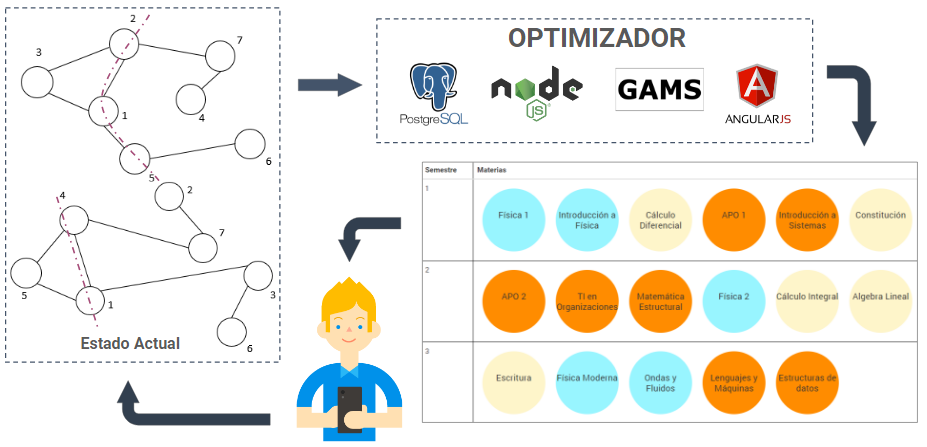
\includegraphics[width=0.45\textwidth]{img/cycle}
    \caption{Cycle}
    \label{cycle}
\end{figure}

%The results showed by the web app can be seen in Figure \ref{fig_results}.
%\begin{figure}[h!]
%\centering
%\includegraphics[width=0.45\textwidth]{img/webapp2}
%\caption{Screenshot of results obtained in web app}
%\label{fig_results}
%\end{figure}

\section{Conclusions and Future Work }

\subsection{Conclusions}

This project leaves the following conclusions:\\

\begin{itemize}
    \item We created an application that minimizes the number of semester a student needs to finish any combination of majors and minors and offer a detailed plan semester by semester of which courses to enroll in each period. \\
    \item Using the capabilities of GAMS and the theory learned about MIP problems optimization, it was possible to make a boring and time-consuming task in a matter of seconds.\\
    \item The course offer for each semester is not an easy task for the university because they have to estimate based on previous years what classes the students want to take. It often happens that the university need more or less courses, which translates into money loss. With this solution they could get a better estimate of the classes that students want to take. \\
\end{itemize}

\subsection{Future Work}
As for future work we have several ideas to improve our implementation of the solution. These are:\\

\begin{itemize}
    \item Fill the database with all the majors and minors offered by Uniandes. Specially, try to find an automatic way to do it by talking to the university.\\ 
    \item Implement user accounts so that each student preferences are saved. \\
    \item Implement program coordinators' accounts, so that for each program the its coordinator can update information and add specific restrictions that don't apply to the whole university.\\
    \item Integration with next semester schedule, so users can find courses with their preferred hours. Specially, so that the application doesn't suggest combinations that cannot happen due to courses that overlap in their schedules.\\
    \item Automatic integration of new courses, to make the application easily scalable.\\
\end{itemize}

As for the final future work idea, we would like to implement this software in other universities, after finishing the user tests at Uniandes. \\

\section*{Acknowledgments}
The authors would like to thank the professor Yezid Donoso for his counseling in the objective function definition and the license to test and use non-demo solvers. Also to the teaching assistant German Montoya for his help with the GAMS implementation. \\ 

%\newpage
%\appendices
%\section{Test Cases}
%Test case for Systems and computing engineering undergraduate program
%\begin{figure}[h!]
%\centering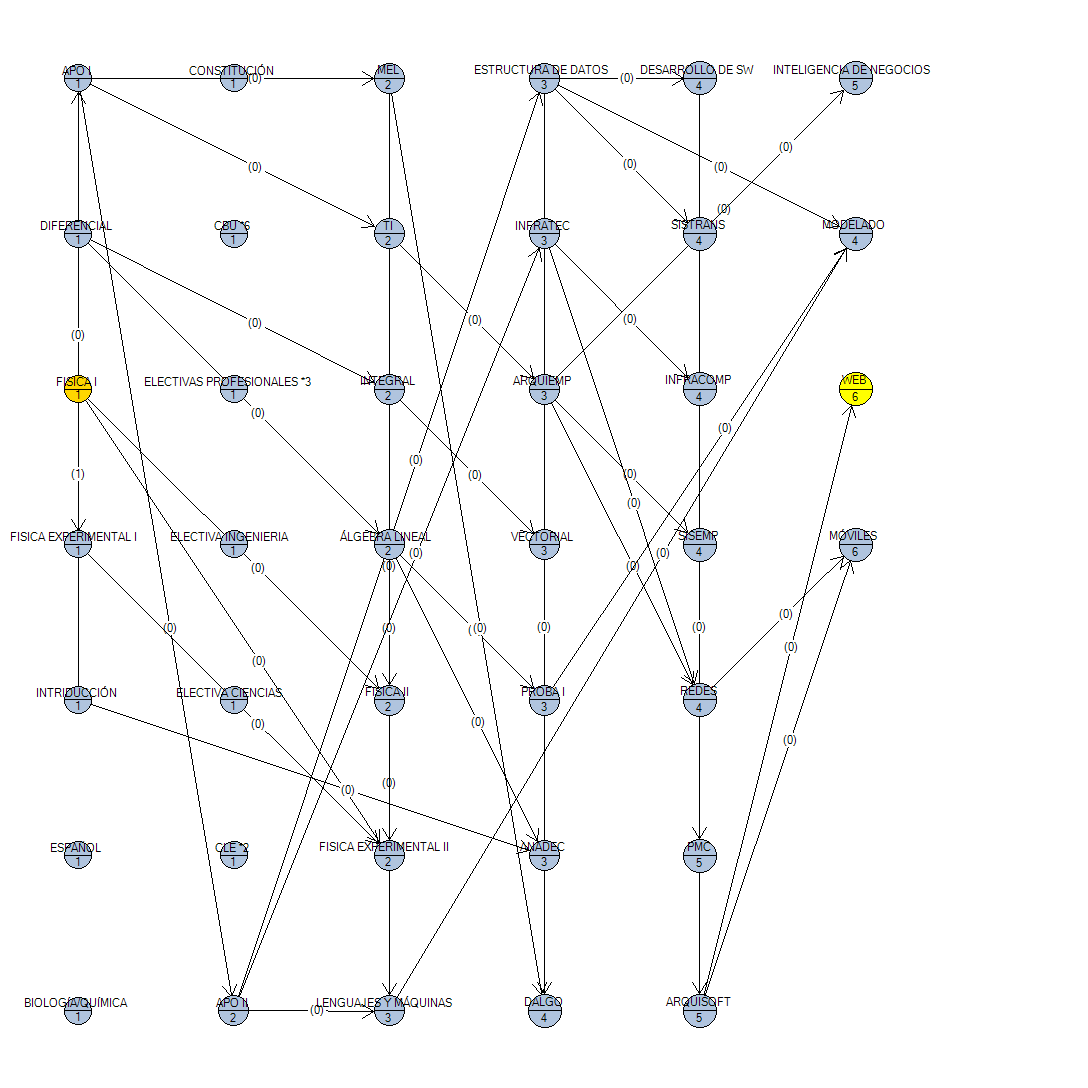
\includegraphics[width=\textwidth]{img/grafo_sistemas.png}
%\caption{Systems and computing engineering graph}
%\label{grafo_sistemas}
%\end{figure}
%\clearpage
%Test case for Physics undergraduate program
%\begin{figure}[h!]
%\centering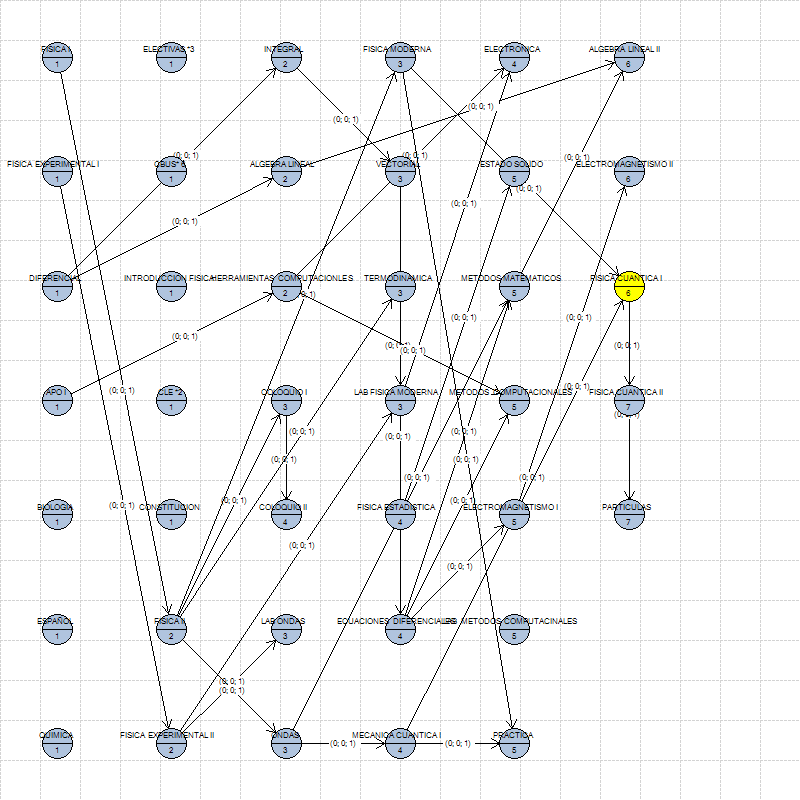
\includegraphics[width=\textwidth]{img/grafo_fisica.png}
%\caption{Physics graph}
%\label{grafo_fisica}
%\end{figure}
%\clearpage

% can use a bibliography generated by BibTeX as a .bbl file
% BibTeX documentation can be easily obtained at:
% http://www.ctan.org/tex-archive/biblio/bibtex/contrib/doc/
% The IEEEtran BibTeX style support page is at:
% http://www.michaelshell.org/tex/ieeetran/bibtex/
\bibliographystyle{IEEEtran}
\bibliography{references}

\end{document}


